% Source PDF page 593 (printed p. 579)
\section{可行性与第一阶段方法}
障碍法需要严格可行初始点 $x^{(0)}$。如果不知道这样的点，则先进行一个称为\emph{第一阶段}的预备过程，计算严格可行点，或确定约束不可行。然后将第一阶段得到的严格可行点作为障碍法的初始点，此时的障碍法称为\emph{第二阶段}。本节介绍几种第一阶段方法。

\subsection{基本的第一阶段方法}
考虑关于变量 $x\in\R^n$ 的一组不等式与等式
\begin{equation}
f_i(x)\le0,\quad i=1,\ldots,m,\qquad Ax=b,\tag{11.18}
\end{equation}
其中 $f_i:\R^n\to\R$ 为凸函数，具有连续的二阶导数。假设已给定点 $x^{(0)}\in\dom f_1\cap\cdots\cap\dom f_m$，满足 $Ax^{(0)}=b$。

我们的目标是找到严格满足这些不等式与等式的解，或判定不存在这样的解。为此构造优化问题
\begin{equation}\begin{aligned}
\text{最小化}\quad&s\\
\text{约束为}\quad&f_i(x)\le s,\quad i=1,\ldots,m,\\
&Ax=b,
\end{aligned}\tag{11.19}\end{equation}
变量为 $x\in\R^n$、$s\in\R$。变量 $s$ 可解释为不等式最大违反程度的上界；目标是将最大违反程度降到零以下。

这个问题总是严格可行，因为可以选 $x^{(0)}$ 作为 $x$ 的初始点，并选任意大于 $\max_{i=1,\ldots,m}f_i(x^{(0)})$ 的数作为 $s$。因此，可以应用障碍法求解 (11.19)，它称为不等式与等式系统 (11.19) 对应的第一阶段优化问题。

根据 (11.19) 最优值 $\bar p^\star$ 的正负，可以分为三种情况。
\begin{enumerate}
\item 若 $\bar p^\star<0$，则 (11.18) 有严格可行解。而且，若 $(x,s)$ 对 (11.19) 可行且 $s<0$，则 $x$ 满足 $f_i(x)<0$。这意味着不必高精度求解优化问题 (11.19)，在 $s<0$ 时即可终止。
\item 若 $\bar p^\star>0$，则 (11.18) 不可行。与情况1一样，无须高精度求解第一阶段优化问题 (11.19)：找到对偶目标为正的对偶可行点时即可终止，因为这证明 $\bar p^\star>0$。此时可以根据对偶可行点，构造证明 (11.18) 不可行的择一系统的解。
\item 若 $\bar p^\star=0$，且最小值在 $x^\star$、$s^\star=0$ 处取得，则该不等式组可行，但不严格可行。若 $\bar p^\star=0$，但最小值未取得，则不等式组不可行。
% Source PDF page 594 (printed p. 580)
实际中不可能精确判定 $\bar p^\star=0$。应用于 (11.19) 的优化算法会以 $|\bar p^\star|<\epsilon$ 的结论终止，其中 $\epsilon$ 是某个很小的正数。这使我们能够断定，不等式组 $f_i(x)\le-\epsilon$ 不可行，而不等式组 $f_i(x)\le\epsilon$ 可行。
\end{enumerate}

\subsubsection*{违反程度之和}
刚介绍的基本第一阶段方法有许多变体。一种方法最小化违反程度之和，而非最大违反程度。构造问题
\begin{equation}\begin{aligned}
\text{最小化}\quad&\one^\T s\\
\text{约束为}\quad&f_i(x)\le s_i,\quad i=1,\ldots,m,\\
&Ax=b,\\&s\succeq0.
\end{aligned}\tag{11.20}\end{equation}
固定 $x$ 时，$s_i$ 的最优值为 $\max\{f_i(x),0\}$，所以这个问题是在最小化违反程度之和。(11.20) 的最优值为零且能取得，当且仅当原来的等式与不等式组可行。

当等式与不等式系统 (11.19) 不可行时，这个违反程度之和第一阶段方法有一个很有意思的性质。第一阶段问题 (11.20) 的最优点通常只违反很少的几个不等式，设为 $r$ 个。因此，我们计算出了一个满足很多（$m-r$ 个）不等式的点，也就是识别出一个很大的可行不等式子集。此时，严格满足的不等式对应的对偶变量为零，因而还证明了某个不等式子集不可行。这比只知道全部 $m$ 个不等式合在一起不可行，提供了更多信息。（这一现象与寻找稀疏近似解时采用的 $\ell_1$ 范数正则化或基追踪密切相关；见第6.1.2节和第6.5.4节。）

\begin{origexample}{11.4}
\emph{第一阶段方法的比较。} 对一个不可行不等式组 $Ax\preceq b$ 应用两种第一阶段方法，维数为 $m=100$、$n=50$。第一种是基本第一阶段方法
\[
\begin{aligned}\text{最小化}\quad&s\\\text{约束为}\quad&Ax\preceq b+\one s,\end{aligned}
\]
它最小化最大违反程度。第二种最小化违反程度之和，即求解 LP
\[
\begin{aligned}\text{最小化}\quad&\one^\T s\\\text{约束为}\quad&Ax\preceq b+s,\\&s\succeq0.\end{aligned}
\]
这两种方法求得的 $x$ 分别记为 $x_{\mathrm{max}}$、$x_{\mathrm{sum}}$。图11.9给出了两者的违反程度 $b_i-a_i^\T x$ 的分布。点 $x_{\mathrm{max}}$ 满足 $100$ 个不等式中的 $39$ 个，而 $x_{\mathrm{sum}}$ 满足其中 $79$ 个。
\end{origexample}

% Source PDF page 595 (printed p. 581)
\begin{figure}[htbp]\centering
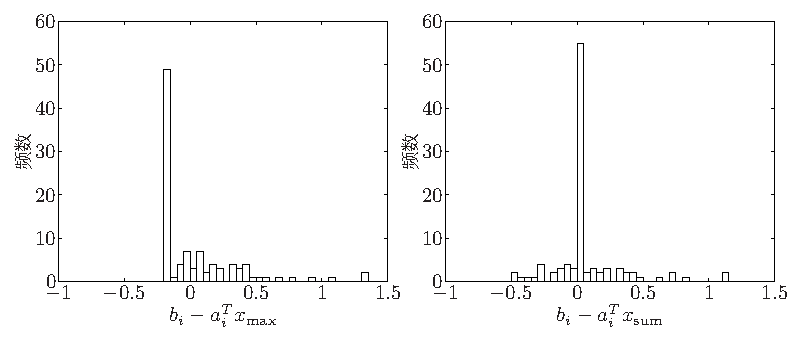
\includegraphics[width=.95\textwidth]{figures/ch11-09.pdf}
\caption*{图11.9 一个含 $100$ 个不等式 $a_i^\T x\le b_i$、$50$ 个变量的不可行不等式组，其违反程度 $b_i-a_i^\T x$ 的分布。左图的 $x_{\mathrm{max}}$ 由基本第一阶段算法得到，它满足 $100$ 个不等式中的 $39$ 个。右图的 $x_{\mathrm{sum}}$ 通过最小化违反程度之和得到，它满足 $100$ 个不等式中的 $79$ 个。}
\end{figure}
\subsubsection*{在第二阶段中心路径附近终止}
使用障碍法的基本第一阶段方法有一个简单变体，具有如下性质：当等式与不等式组严格可行时，第一阶段问题的中心路径与原优化问题 (11.1) 的中心路径相交。

假设给定点 $x^{(0)}\in\mathcal D=\dom f_0\cap\dom f_1\cap\cdots\cap\dom f_m$，且 $Ax^{(0)}=b$。构造第一阶段优化问题
\begin{equation}\begin{aligned}
\text{最小化}\quad&s\\
\text{约束为}\quad&f_i(x)\le s,\quad i=1,\ldots,m,\\
&f_0(x)\le M,\\&Ax=b,
\end{aligned}\tag{11.21}\end{equation}
其中常数 $M$ 取为大于 $\max\{f_0(x^{(0)}),p^\star\}$。

现在假设原问题 (11.1) 严格可行，于是 (11.21) 的最优值 $\bar p^\star$ 为负。问题 (11.21) 的中心路径由下列条件刻画：
\[
\sum_{i=1}^m\frac1{s-f_i(x)}=\bar t,\qquad
\frac{\nabla f_0(x)}{M-f_0(x)}+\sum_{i=1}^m\frac{\nabla f_i(x)}{s-f_i(x)}+A^\T\nu=0,
\]
其中 $\bar t$ 为参数。若 $(x,s)$ 在中心路径上且 $s=0$，则 $x$ 和 $\nu$ 满足
\[
t\nabla f_0(x)+\sum_{i=1}^m\frac1{-f_i(x)}\nabla f_i(x)+A^\T\nu=0,
\]
其中 $t=1/(M-f_0(x))$。这说明 $x$ 在原优化问题 (11.1) 的中心路径上，
% Source PDF page 596 (printed p. 582)
对应的对偶间隙为
\begin{equation}
m(M-f_0(x))\le m(M-p^\star).\tag{11.22}
\end{equation}

\subsection{用不可行初始点牛顿法实现第一阶段}
也可以对原问题的一个修改版本应用不可行初始点牛顿法，完成第一阶段。原问题为
\[
\begin{aligned}\text{最小化}\quad&f_0(x)\\\text{约束为}\quad&f_i(x)\le0,\quad i=1,\ldots,m,\\&Ax=b.\end{aligned}
\]
首先将问题写成显然等价的形式
\[
\begin{aligned}\text{最小化}\quad&f_0(x)\\\text{约束为}\quad&f_i(x)\le s,\quad i=1,\ldots,m,\\&Ax=b,\qquad s=0,\end{aligned}
\]
其中增加了变量 $s\in\R$。为启动障碍法，用不可行初始点牛顿法求解
\[
\begin{aligned}
\text{最小化}\quad&t^{(0)}f_0(x)-\sum_{i=1}^m\log(s-f_i(x))\\
\text{约束为}\quad&Ax=b,\qquad s=0.
\end{aligned}
\]
可用任意 $x\in\mathcal D$ 以及任意 $s>\max_i f_i(x)$ 初始化。只要问题严格可行，不可行初始点牛顿法最终会采用一个无阻尼步，此后有 $s=0$，即 $x$ 严格可行。

若连这些函数公共定义域 $\mathcal D$ 内的一个点也不知道，同样可以使用这一技巧。只需对问题
\[
\begin{aligned}
\text{最小化}\quad&t^{(0)}f_0(x+z_0)-\sum_{i=1}^m\log(s-f_i(x+z_i))\\
\text{约束为}\quad&Ax=b,\qquad s=0,\qquad z_0=0,\ \ldots,\ z_m=0,
\end{aligned}
\]
应用不可行初始点牛顿法，变量为 $x,z_0,\ldots,z_m$ 以及 $s\in\R$。初始化 $z_i$ 时使 $x+z_i\in\dom f_i$。

用这种方法处理第一阶段问题的主要缺点，是在问题不可行时没有好的停止准则；残差只是无法收敛到零。

\subsection{例子}
考虑一族线性可行性问题
\[
Ax\preceq b(\gamma),
\]
其中 $A\in\R^{50\times20}$，$b(\gamma)=b+\gamma\Delta b$。选取数据，使不等式组在 $\gamma>0$ 时严格可行，$\gamma<0$ 时不可行，$\gamma=0$ 时可行但不严格可行。

% Source PDF page 597 (printed p. 583)
图11.10给出 $\gamma$ 在 $[-1,1]$ 内取 $40$ 个值时，找到严格可行点或不可行证书所需的总牛顿步数。使用第11.4.1节的基本第一阶段方法，即对每个 $\gamma$ 构造 LP
\[
\begin{aligned}\text{最小化}\quad&s\\\text{约束为}\quad&Ax\preceq b(\gamma)+s\one.\end{aligned}
\]
障碍法参数取 $\mu=10$，初始点为 $x=0$、$s=-\min_i b_i(\gamma)+1$。找到满足 $s<0$ 的点 $(x,s)$，或找到对偶问题
\[
\begin{aligned}
\text{最大化}\quad&-b(\gamma)^\T z\\
\text{约束为}\quad&A^\T z=0,\\&\one^\T z=1,\\&z\succeq0
\end{aligned}
\]
的可行解 $z$ 且 $-b(\gamma)^\T z>0$ 时，算法终止。

图中显示，若不等式组具有一定可行余量，约需 $25$ 个牛顿步就能找到严格可行点。反之，若不等式组具有一定不可行余量，则约需 $35$ 步得到证明不可行的证书。当不等式组接近可行与不可行的分界，即 $\gamma$ 接近零时，第一阶段的计算工作量增大。当 $\gamma$ 非常接近零，即不等式组非常接近可行与不可行的分界时，所需步数显著增长。图11.11给出 $\gamma$ 接近零时的总牛顿步数。曲线表明，对于非常接近可行与不可行分界的问题，检测可行性或证明不可行性所需步数近似按对数增长。

这个例子具有代表性：只要问题不十分接近可行与不可行的分界，用障碍法求解凸不等式组与线性等式组的成本就不大，而且近似不变。当问题非常接近分界时，寻找严格可行点或不可行证书所需的牛顿步数增加。当问题恰好位于严格可行与不可行之间的边界上，例如可行但不严格可行时，成本变为无穷大。

\subsubsection*{用不可行初始点牛顿法求可行点}
还对问题
\[
\begin{aligned}\text{最小化}\quad&-\sum_{i=1}^m\log s_i\\\text{约束为}\quad&Ax+s=b(\gamma)\end{aligned}
\]
应用不可行初始点牛顿法，求解同一组可行性问题。

采用回溯参数 $\alpha=0.01$、$\beta=0.9$，初始化 $x^{(0)}=0$、$s^{(0)}=\one$、$\nu^{(0)}=0$。只考察可行问题，即 $\gamma>0$，并在找到可行点时终止。（不考察不可行问题，因为这种情况下残差只会收敛到一个正数。）图11.12给出找到可行点所需牛顿步数随 $\gamma$ 的变化。

% Source PDF page 598 (printed p. 584)
\begin{figure}[htbp]\centering
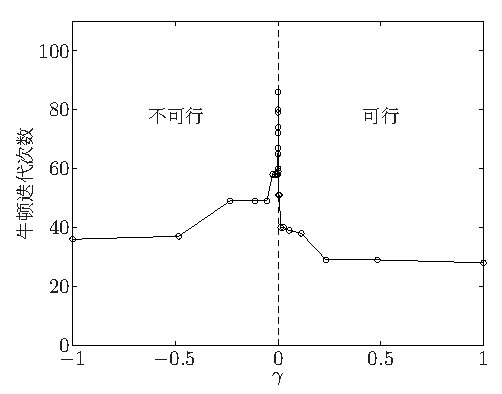
\includegraphics[width=.63\textwidth]{figures/ch11-10.pdf}
\caption*{图11.10 判定由 $\gamma\in\R$ 参数化的线性不等式组 $Ax\preceq b+\gamma\Delta b$ 可行或不可行所需的牛顿迭代次数。不等式组在 $\gamma>0$ 时严格可行，在 $\gamma<0$ 时不可行。$\gamma$ 大于约 $0.2$ 时，计算严格可行点约需 $30$ 步；$\gamma$ 小于约 $-0.5$ 时，产生不可行证书约需 $35$ 步。中间的 $\gamma$ 值，特别是接近零时，需要更多牛顿步才能判定可行性。}
\end{figure}
\begin{figure}[htbp]\centering
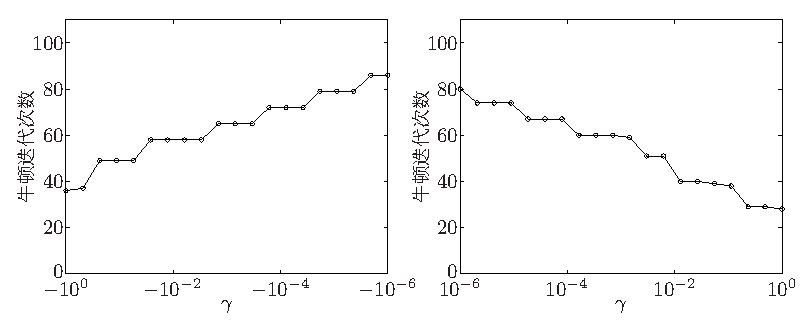
\includegraphics[width=.95\textwidth]{figures/ch11-11.pdf}
\caption*{图11.11 左：$\gamma$ 为很小负数时，找到不可行性证明所需的牛顿迭代次数与 $\gamma$ 的关系。右：$\gamma$ 为很小正数时，找到严格可行点所需的牛顿迭代次数与 $\gamma$ 的关系。}
\end{figure}

% Source PDF page 599 (printed p. 585), conclusion of section 11.4.3.
\begin{figure}[htbp]\centering
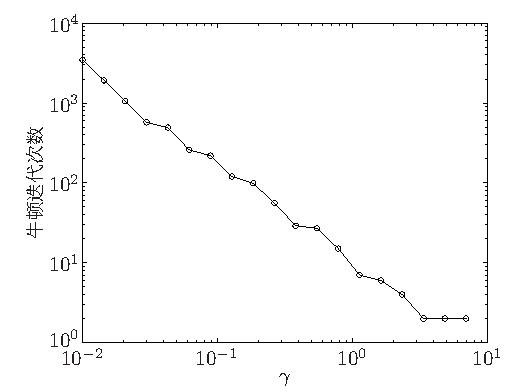
\includegraphics[width=.65\textwidth]{figures/ch11-12.pdf}
\caption*{图11.12 对由 $\gamma\in\R$ 参数化的线性不等式组 $Ax\preceq b+\gamma\Delta b$，找到可行点所需的迭代次数。使用不可行初始点牛顿法，在找到可行点时终止。$\gamma=10$ 时，初始点 $x^{(0)}=0$ 恰好可行，因此无需迭代。}
\end{figure}
图中可见，$\gamma$ 大于约 $0.3$ 时，找到可行点所需的牛顿步数少于 $20$。这些情况下，该方法比总共约需 $30$ 个牛顿步的第一阶段方法更有效。$\gamma$ 更小时，所需牛顿步数急剧增加，近似与 $1/\gamma$ 成正比。$\gamma=0.01$ 时，不可行初始点牛顿法需要几千次迭代才能得到可行点。在这个范围内，第一阶段方法有效得多，仅需约 $40$ 次迭代。

这些结果很有代表性。只要不等式组可行，而且不很接近可行与不可行的分界，不可行初始点牛顿法就效果很好。但当可行集只是勉强非空时，例如本例中 $\gamma$ 很小的情况，第一阶段方法好得多。第一阶段方法的另一个优点，是能妥善处理不可行情形；相比之下，不可行初始点牛顿法只会不收敛。

